\documentclass{article}

\setlength{\topmargin}{-.5in}
\setlength{\oddsidemargin}{.125in}
\setlength{\textwidth}{6.25in}

% page numbering style
\usepackage{fancyhdr}
\pagestyle{fancy}
\renewcommand{\headrulewidth}{0pt}
\fancyhf{}
\fancyfoot[R]{\thepage}
\fancypagestyle{plain}{%
    \renewcommand{\headrulewidth}{0pt}%
    \fancyhf{}%
    \fancyfoot[R]{\thepage}%
}

\usepackage{float}

\usepackage{Sweave}
\begin{document}
\Sconcordance{concordance:report.tex:report.Rnw:%
1 20 1 1 0 2 1 1 12 1 4 1 25 23 1 1 19 2 1 2 2 342 1 1 43 2 1 2 2 2 1 1 %
34 1 22 1 3 4 0 1 2 1 1}





\title{Mathematics Developers Survey 2016}
\author{Nejc Ilenic}
\date{}
\maketitle

\section{Introduction}
Anonymised responses from Stack Overflow Annual Developer Survey are published each year along the results to encourage their further analysis. Being curious about where in the world and in which domain a data scientist should start her/his career, I attempted to answer some of the question by analysing the available dataset.

\vspace{2mm}

An important thing to note when interpreting the results however is that this data may not be a represantative sample from the population of mathematics developers. One should keep in mind that these are developers who were aware of the survey and were willing to answer the questions.

\section{Data preparation}
The dataset was constructed from survey that took place from January 7 to January 25, 2016, with responses originating from Stack Overflow, Stack Exchange technical sites, Facebook and Twitter. Most of the questions were demographic and regarding professional work and technology. Raw data consists of 56030 samples and 66 features, all of which are optional.

In order to obtain an adequately sizable sample, I have decided to include all respondents that belong to the occupation group of mathematics developers, which includes data scientists, machine learning developers and developers with statistics and mathematics backgrounds. After filtering out other occupations and responses with unknown countries we are left with 2132 samples.

\section{Exploratory analysis}
todo

\subsection{Job satisfaction per country}
Number of mathematics developers per country can be seen in Figure \ref{fig_0}. Minimum number of 40 respondents is required to take the country into account and all others are placed into a single group called \textit{Other}. Note that selected countries and number of people may be different when doing inference of specific features due to missing values (i.e. optional answers in the survey). Majority of respondents are from United States, followed by a combination of countries with less than 40 developers, United Kingdom, Germany and India.


\begin{figure}[H]
\centering
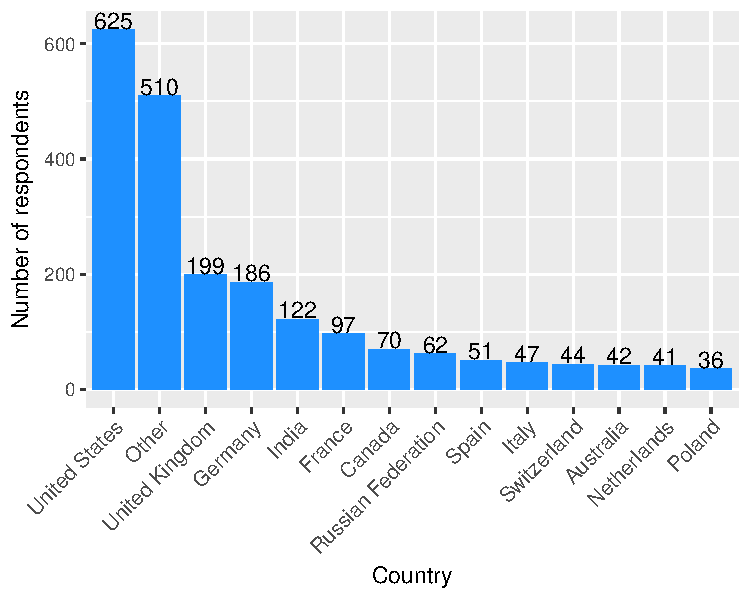
\includegraphics{report-005}
\caption{Number of mathematics developers per country.}\label{fig_0}
\end{figure}

todo





\begin{figure}[H]
\centering
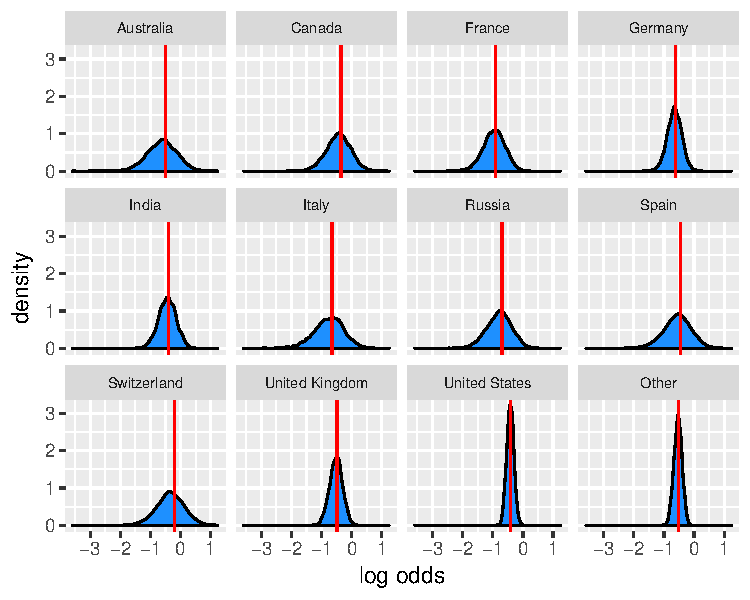
\includegraphics{report-010}
\caption{todo.}\label{fig_1}
\end{figure}


\begin{figure}[H]
\centering
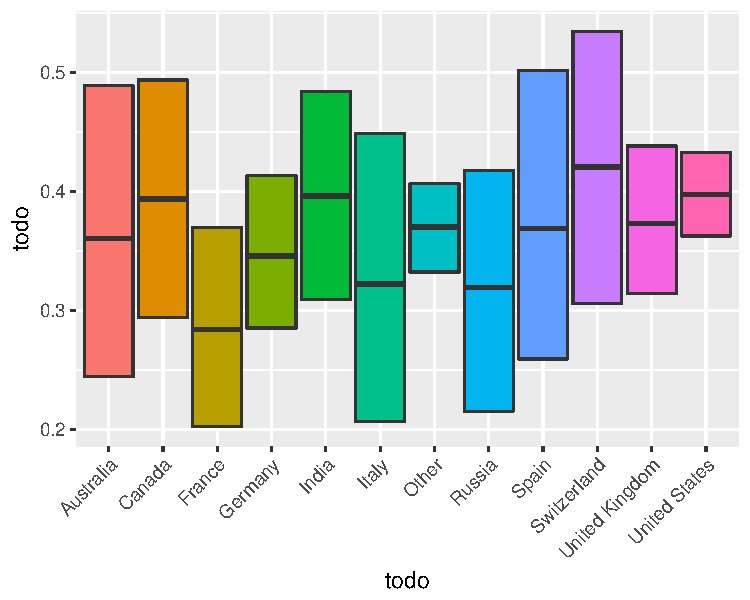
\includegraphics{report-012}
\caption{todo.}\label{fig_2}
\end{figure}

\subsection{Effects on job satisfaction}
todo





\begin{figure}[H]
\centering
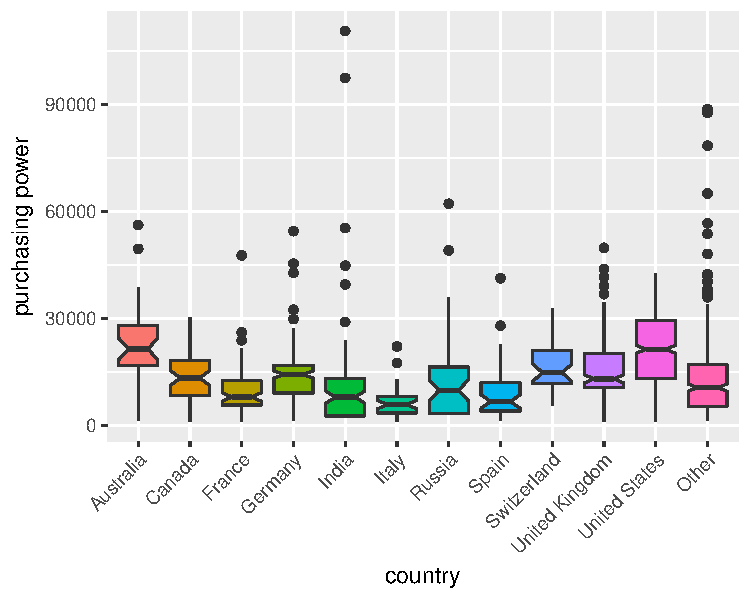
\includegraphics{report-017}
\caption{todo.}\label{fig_3}
\end{figure}


\begin{figure}[H]
\centering
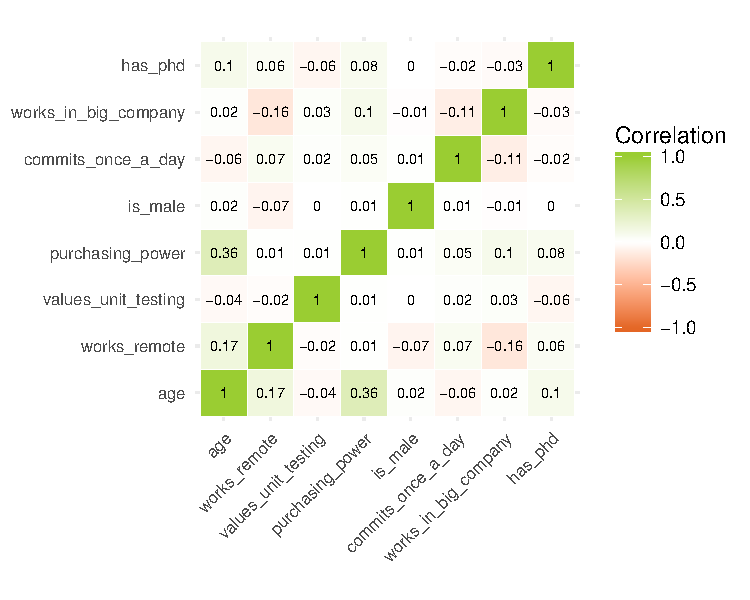
\includegraphics{report-019}
\caption{todo.}\label{fig_4}
\end{figure}


\begin{figure}[H]
\centering
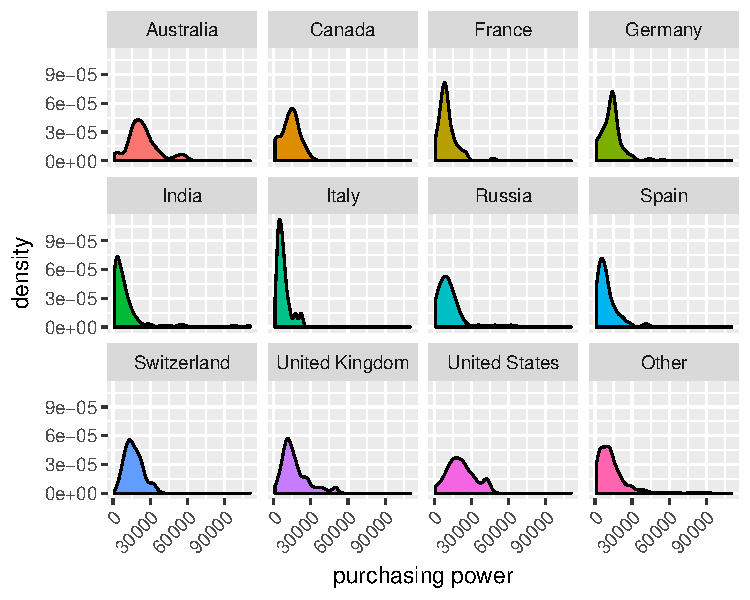
\includegraphics{report-021}
\caption{todo.}\label{fig_5}
\end{figure}

\subsection{Purchasing power per country}
todo


\begin{figure}[H]
\centering
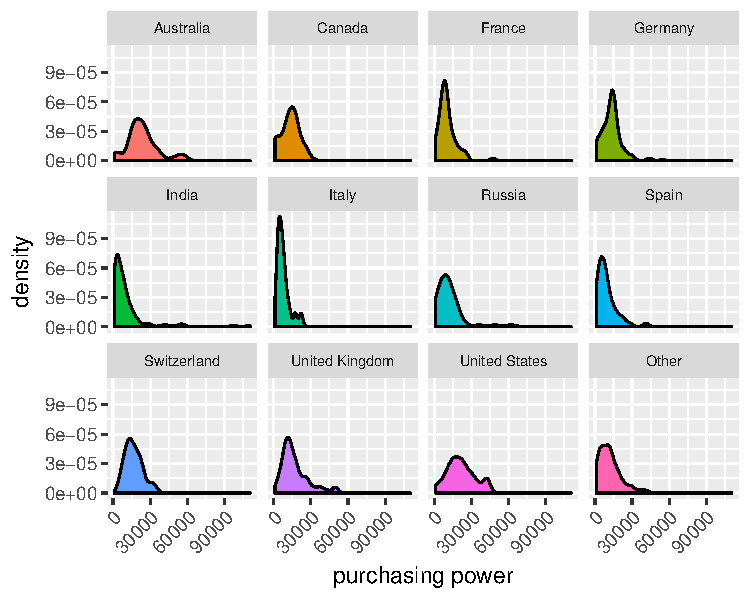
\includegraphics{report-023}
\caption{todo.}\label{fig_6}
\end{figure}




\begin{figure}[H]
\centering
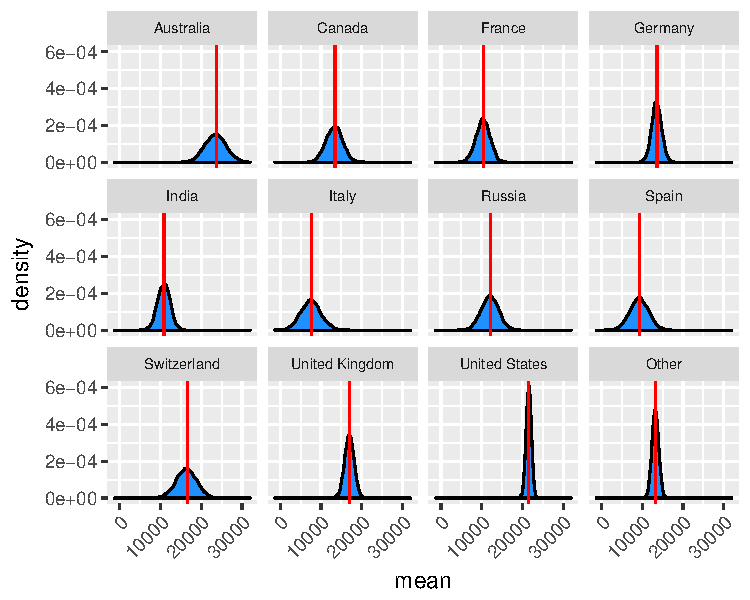
\includegraphics{report-027}
\caption{todo.}\label{fig_7}
\end{figure}


\begin{figure}[H]
\centering
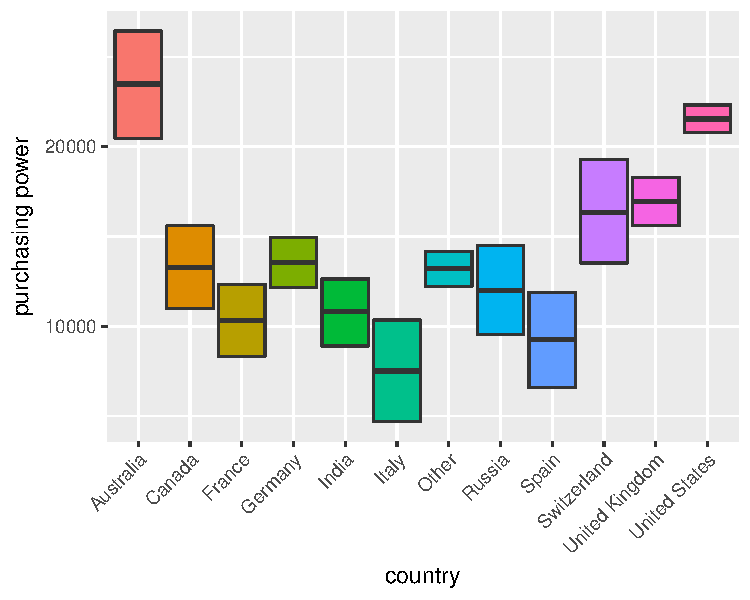
\includegraphics{report-029}
\caption{todo.}\label{fig_8}
\end{figure}

\subsection{Job satisfaction per industry}
todo


\begin{figure}[H]
\centering
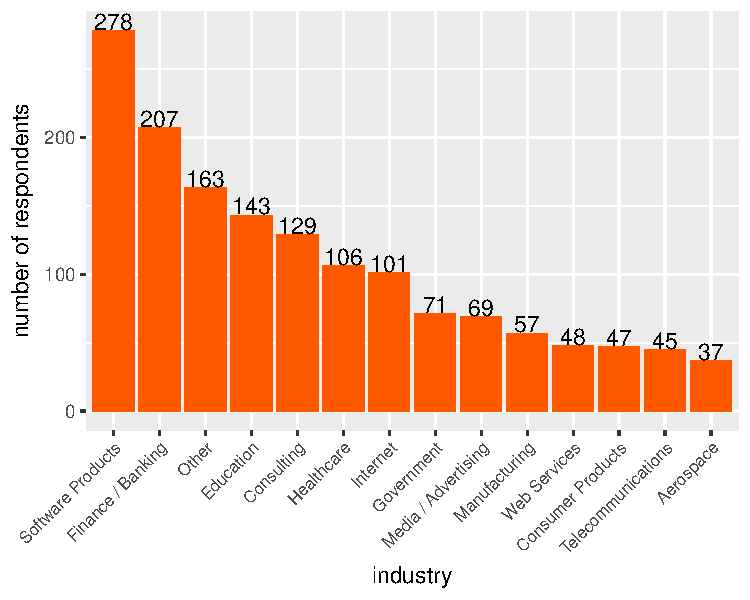
\includegraphics{report-031}
\caption{Number of mathematics developers per industry.}\label{fig_9}
\end{figure}





\begin{figure}[H]
\centering
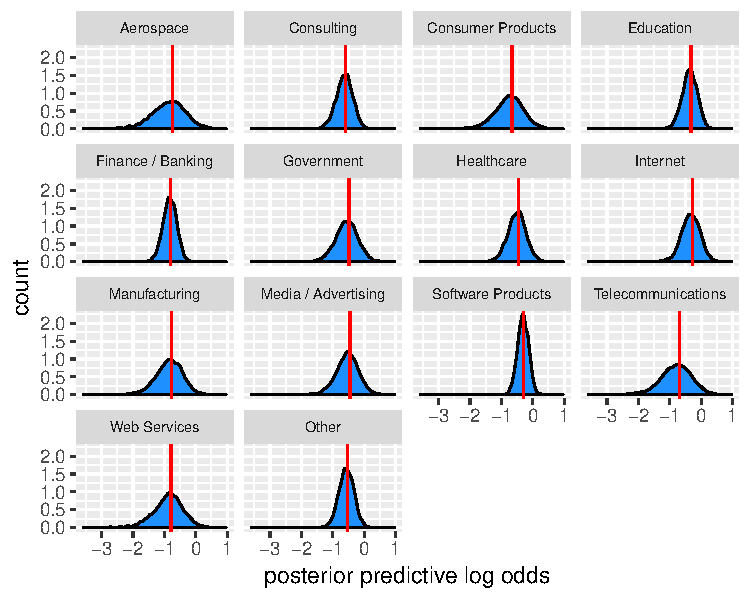
\includegraphics{report-036}
\caption{todo.}\label{fig_10}
\end{figure}


\begin{figure}[H]
\centering
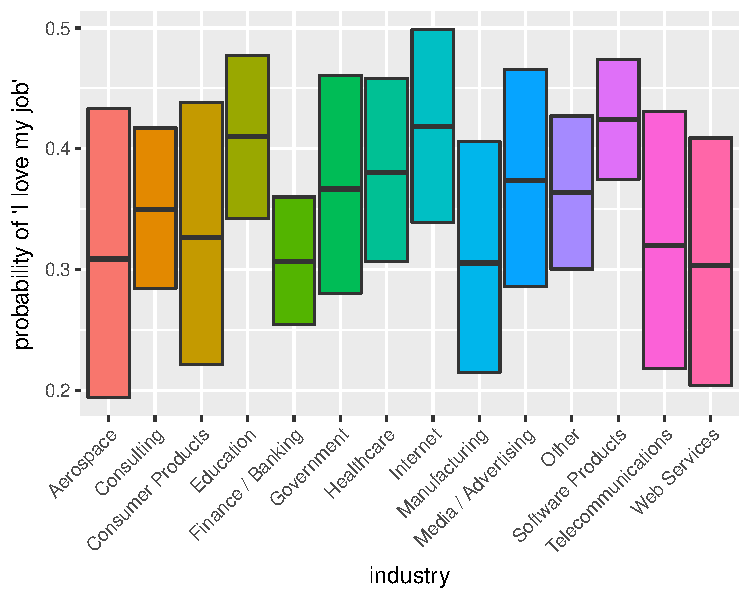
\includegraphics{report-038}
\caption{todo.}\label{fig_11}
\end{figure}

\subsection{Purchasing power per industry}
todo


\begin{figure}[H]
\centering
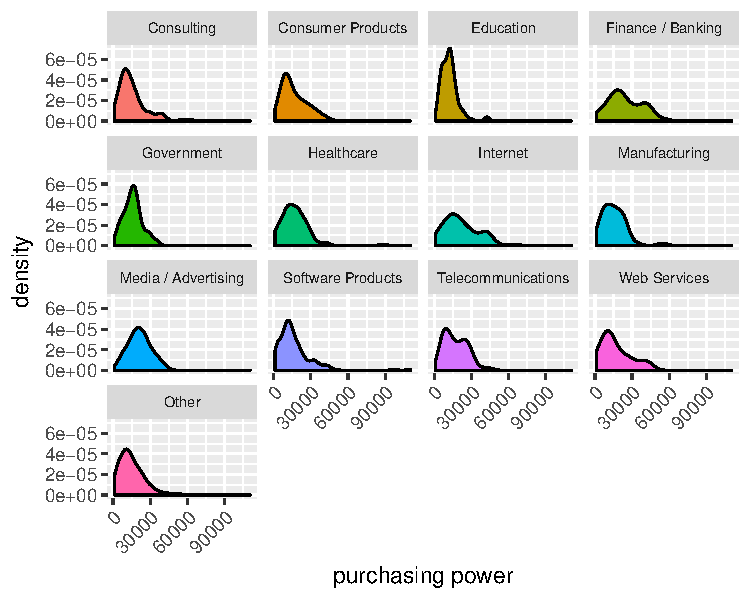
\includegraphics{report-040}
\caption{todo.}\label{fig_12}
\end{figure}




\begin{figure}[H]
\centering
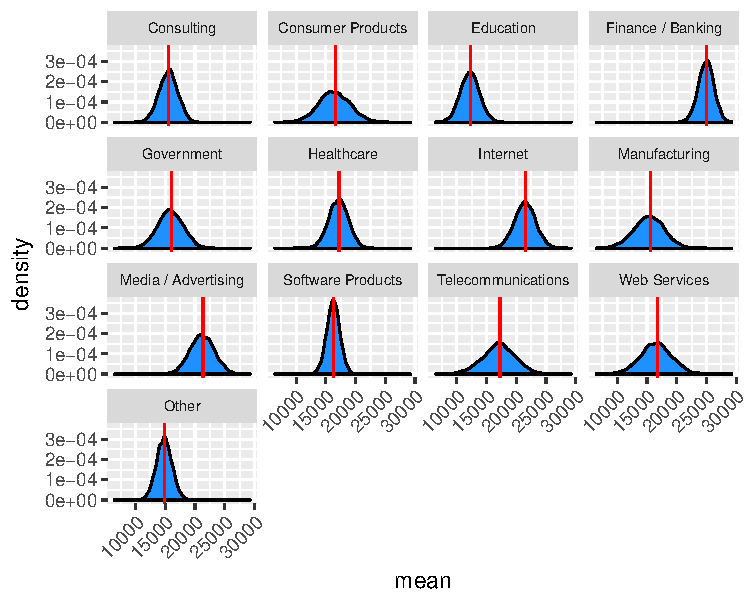
\includegraphics{report-044}
\caption{todo.}\label{fig_13}
\end{figure}


\begin{figure}[H]
\centering
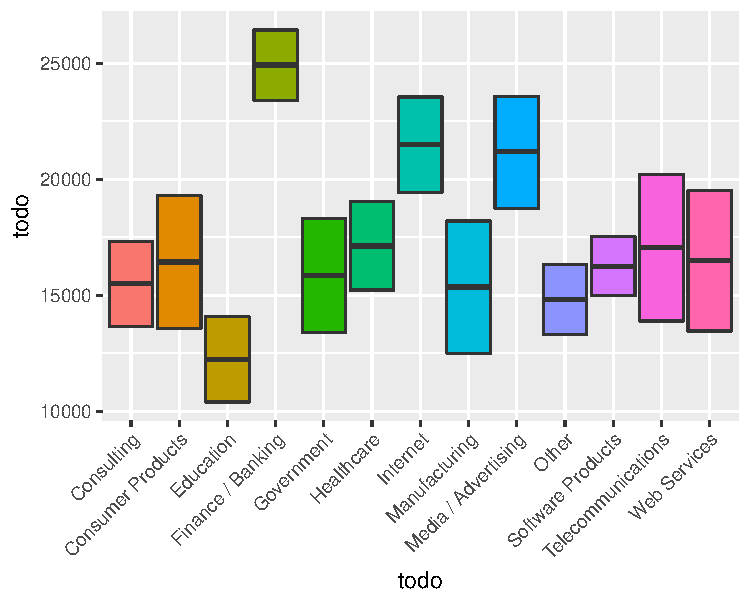
\includegraphics{report-046}
\caption{todo.}\label{fig_14}
\end{figure}

\section{Conclusion}
todo

\end{document}
